\documentclass[11pt]{article}
\usepackage{amssymb, amsthm, amsmath}
\usepackage{bm}
\usepackage{graphicx}
\usepackage[authoryear]{natbib}
\usepackage{bm}
\usepackage{verbatim}
\usepackage{lineno}
\usepackage{times}
\usepackage{soul}
\usepackage{color}
\usepackage{enumitem}
\usepackage{setspace}
\usepackage{times}
\usepackage{changepage}

\usepackage[left=1in,top=1in,right=1in]{geometry}
\pdfpageheight 11in
\pdfpagewidth 8.5in
\linespread{2.0}
\newcommand{\btheta}{ \mbox{\boldmath $\theta$}}
\newcommand{\bmu}{ \mbox{\boldmath $\mu$}}
\newcommand{\balpha}{ \mbox{\boldmath $\alpha$}}
\newcommand{\bbeta}{ \mbox{\boldmath $\beta$}}
\newcommand{\bdelta}{ \mbox{\boldmath $\delta$}}
\newcommand{\blambda}{ \mbox{\boldmath $\lambda$}}
\newcommand{\bgamma}{ \mbox{\boldmath $\gamma$}}
\newcommand{\brho}{ \mbox{\boldmath $\rho$}}
\newcommand{\bpsi}{ \mbox{\boldmath $\psi$}}
\newcommand{\bepsilon}{ \mbox{\boldmath $\epsilon$}}
\newcommand{\bomega}{ \mbox{\boldmath $\omega$}}
\newcommand{\bOmega}{ \mbox{\boldmath $\Omega$}}
\newcommand{\bDelta}{ \mbox{\boldmath $\Delta$}}
\newcommand{\bSigma}{ \mbox{\boldmath $\Sigma$}}
\newcommand{\bPsi}{\mbox{\boldmath $\Psi$}}
\newcommand{\bOne}{\mbox{\boldmath $1$}}
\newcommand{\omu}{\overline{\mu}}
\newcommand{\oSigma}{\overline{\Sigma}}
\newcommand{\Yt}{{\tilde Y}}
\newcommand{\bA}{ \mbox{\bf A}}
\newcommand{\bP}{ \mbox{\bf P}}
\newcommand{\bx}{ \mbox{\bf x}}
\newcommand{\bX}{ \mbox{\bf X}}
\newcommand{\bB}{ \mbox{\bf B}}
\newcommand{\bT}{ \mbox{\bf T}}
\newcommand{\bZ}{ \mbox{\bf Z}}
\newcommand{\by}{ \mbox{\bf y}}
\newcommand{\bY}{ \mbox{\bf Y}}
\newcommand{\bz}{ \mbox{\bf z}}
\newcommand{\bh}{ \mbox{\bf h}}
\renewcommand{\bm}{ \mbox{\bf m}}
\newcommand{\br}{ \mbox{\bf r}}
\newcommand{\bt}{ \mbox{\bf t}}
\newcommand{\bk}{\mbox{\bf k}}
\newcommand{\bs}{ \mbox{\bf s}}
\newcommand{\bb}{ \mbox{\bf b}}
\newcommand{\bL}{ \mbox{\bf L}}
\newcommand{\bu}{ \mbox{\bf u}}
\newcommand{\bv}{ \mbox{\bf v}}
\newcommand{\bV}{ \mbox{\bf V}}
\newcommand{\bW}{ \mbox{\bf W}}
\newcommand{\bG}{ \mbox{\bf G}}
\newcommand{\bH}{ \mbox{\bf H}}
\newcommand{\bw}{ \mbox{\bf w}}
\newcommand{\bo}{ \mbox{\bf o}}
\newcommand{\bfe}{ \mbox{\bf e}}
\newcommand{\iid}{\stackrel{iid}{\sim}}
\newcommand{\ind}{\stackrel{ind}{\sim}}
\newcommand{\dd}{\; \text{d} }
\newcommand{\ddd}{\text{d} }
\newcommand{\indep}{\stackrel{indep}{\sim}}
\newcommand{\converged}{\stackrel{d}{\rightarrow}}
\newcommand{\goesto}[1]{\stackrel[#1]{}{\longrightarrow}}
\newcommand{\calR}{{\cal R}}
\newcommand{\calG}{{\cal G}}
\newcommand{\calD}{{\cal D}}
\newcommand{\calS}{{\cal S}}
\newcommand{\calB}{{\cal B}}
\newcommand{\calA}{{\cal A}}
\newcommand{\calT}{{\cal T}}
\newcommand{\calO}{{\cal O}}
\newcommand{\argmax}{{\mathop{\rm arg\, max}}}
\newcommand{\argmin}{{\mathop{\rm arg\, min}}}
\newcommand{\Frechet}{\mbox{Fr$\acute{\mbox{e}}$chet }}
\newcommand{\Matern}{\mbox{Mat$\acute{\mbox{e}}$rn }}
\newcommand{\ballunion}{B_a(\bs_1) \cup B_b(\bs_2) }

\newcommand{\alphahat}{\hat{\alpha}}

\newcommand{\eref}[1]{(\ref{#1})}
\newcommand{\fref}[1]{Figure~\ref{#1}}
\newcommand{\tref}[1]{Table~\ref{#1}}
\newcommand{\sref}[1]{Section~\ref{#1}}
\newcommand{\aref}[1]{Appendix~\ref{#1}}

\newcommand{\beq}{ \begin{equation}}
\newcommand{\eeq}{ \end{equation}}
\newcommand{\beqn}{ \begin{eqnarray}}
\newcommand{\eeqn}{ \end{eqnarray}}

\newcommand*\patchAmsMathEnvironmentForLineno[1]{%
  \expandafter\let\csname old#1\expandafter\endcsname\csname #1\endcsname
  \expandafter\let\csname oldend#1\expandafter\endcsname\csname end#1\endcsname
  \renewenvironment{#1}%
     {\linenomath\csname old#1\endcsname}%
     {\csname oldend#1\endcsname\endlinenomath}}% 
\newcommand*\patchBothAmsMathEnvironmentsForLineno[1]{%
  \patchAmsMathEnvironmentForLineno{#1}%
  \patchAmsMathEnvironmentForLineno{#1*}}%
\AtBeginDocument{%
\patchBothAmsMathEnvironmentsForLineno{equation}%
\patchBothAmsMathEnvironmentsForLineno{align}%
\patchBothAmsMathEnvironmentsForLineno{flalign}%
\patchBothAmsMathEnvironmentsForLineno{alignat}%
\patchBothAmsMathEnvironmentsForLineno{gather}%
\patchBothAmsMathEnvironmentsForLineno{multline}%
}



\begin{document}\linenumbers
\pagestyle{empty}
\begin{center}
{\Large {\bf PCA for extremes}}\\

{\large Sam Morris\footnote[1]{North Carolina State University}, Brian J Reich\footnotemark[1]{}, Emeric Thibauld\footnote[2]{Colorado State University}, and Dan Cooley\footnotemark[2]{}}

%\footnote{This is the footnote} looks like this. Later text referring to same footnote\footnotemark[\value{footnote}]
\today
\end{center}


\begin{abstract}
	words...\\
	{\bf Key words}: Max-stable process.

\end{abstract}
\newpage
\pagestyle{plain}
\setcounter{page}{1}

\section{Introduction}\label{s:intro}

\section{Model}\label{s:model}


Let $Y_{it}$ be the observation at location $\bs_i$ for $i\in\{1,...,n_s\}$ and time $t\in\{1,...,n_t\}$.  To focus attention on the extreme values, we consider data above a threshold $T$.  The marginal distribution of $Y_{it}$ is then determined by the probability of exceeding the threshold and the distribution of the excursions. Denote the exceedance probability as Prob$[Y_{it}>T] = p_{it}$.  Extreme value theory says that for sufficiently large $T$ the excursion distribution can be approximated using a generalized Pareto distribution (GPD).  Therefore we model $Y_{it}|Y_{it}>T \sim$ GDP$(\sigma_{it},\xi)$, where the GDP  scale and shape parameters are denoted $\sigma_{it}>0$ and $\xi$, respectively.

{\bf spectral, max-linear...finally we settle on...} Spatial extremal dependence is captured using a max-stable copula (define).  Let $Z_{it}$ be a max-stable process with $\Frechet$ marginal distributions (define GEV etc...).  Our objective is to identify a low-rank model for spatial dependence in $Z_{it}$.  Decompose  $Z_{it}$ as $Z_{it}=\theta_{it}\varepsilon_{it}$ where $\theta_{it}$ is a spatial process and $\varepsilon_{it}\iid$ GEV$(1,\alpha,\alpha)$ is a nugget.  The spatial component is written as a combination of $L$ basis functions $B_{il}$
\beq \label{theta}
  \theta_{it} = \left(\sum_{l=1}^LB_{il}^{1/\alpha}A_{lt}\right)^{\alpha}.
\eeq
If $B_{il}>0$, $\sum_{l=1}^LB_{il}=1$, and the $A_{lt}$ have positive stable (PS) distribution $A_{lt}\sim$ PS$(\alpha)$ (define), then $Z_{it}$ is max-stable and has $\Frechet$ marginal distributions.

The $Z_{it}$ are conditionally independent given the spatial random effects, with conditional distribution $Z_{it}|\theta_{it}\sim$.  As a result, the likelihood is $Y_{it}|\theta_{it} \indep g(y;\theta_{it},p_{it},\sigma_{it},\xi)$ where
\beq\label{g}
   g(y;\theta,p,\sigma,\xi)  =
\eeq
Therefore, the likelihood factors across observations which is computationally convenient. Marginalizing over the random effect $\theta_{it}$ induces extremal spatial dependence in the $Z_{it}$, and thus the $Y_{it}$.   Spatial dependence can be summarized by the extremal coefficient (EC) $\vartheta_{ij}\in[1,2]$, where
\beq\label{ECdev}
  \mbox{Prob}(Z_{it}<c,Z_{jt}<c) = \mbox{Prob}(Z_{it}<c)^{\vartheta_{ij}}.
\eeq

For the PS random effects model the EC has the form
\beq\label{EC}
   \vartheta_{ij} = \sum_{l=1}^L \left(B_{il}^{1/\alpha}+B_{jl}^{1/\alpha}\right)^\alpha.
\eeq
In particular, $\vartheta_{ii} = 2^{\alpha}$ for all $i$.  Since $\sum_{l=1}^LB_{il}=1$ for all $i$, we have $\sum_{l=1}^L(\sum_{i=1}^{n_s}B_{il}/n_s) = 1$.  Therefore, the relative contribution of term $l$ can be measured by
\beq
  v_l = \sum_{i=1}^{n_s}B_{il}/n_s,
\eeq
with $\sum_{l=1}^Lv_l=1$.  The order of the terms is arbitrary, and so we assume without loss of generality that $v_1\ge...\ge v_L$.


\section{Estimating the extremal coefficient function}\label{s:estimation}

In this section we develop an algorithm to estimate the spatial dependence parameter $\alpha$ and the $n_s\times L$ matrix $\bB = \{B_{il}\}$.  Given these parameters, we plug them into our model and proceed with Bayesian analysis as described in Section \ref{s:MCMC}.  Our algorithm has the following steps:
\begin{itemize}
  \item[] (1) Obtain an initial estimate of the extremal coefficient for each pair of locations, ${\hat \vartheta}_{ij}$.
  \item[] (2) Spatially smooth these initial estimates ${\hat \vartheta}_{ij}$ using kernel smoothing to obtain ${\tilde \vartheta}_{ij}$.
  \item[] (3) Estimate the spatial dependence parameters by minimizing the difference between model-based coefficients, $\vartheta_{ij}$, and smoothed coefficients, ${\tilde \vartheta}_{ij}$.
\end{itemize}

To estimate the spatial dependence we first remove variation in the marginal distribution through a sample rank transformation so that the marginal distribution at each location is approximately uniform.
Let $U_{it} = r_t(\bY_{i})/(n_t + 1)$, where $r_t(\bY_{i})$ is the sample rank of the $t$th entry of $\bY_{i}$.
Then for some extreme probability $q\in(0,1)$, solving (\ref{ECdev}) suggest the estimate
\beq\label{EChat0}
   {\hat \vartheta}_{ij}(q) = \frac{\log[Q_{ij}(q)]}{\log(q)},
\eeq
where $Q_{ij}(q) = \sum_{t=1}^{n_t}I[U_{it}<q,U_{jt}<q]/n_t$ is the sample proportion of the time points at which both sites are less then $q$.
Since all large $q$ give valid estimates, we average over a grid of $q$ with $q_1<\cdots<q_{n_q}$
\beq\label{EChat1}
{\hat \vartheta}_{ij} = \frac{1}{n_q}\sum_{j=1}^{n_q}{\hat \vartheta}_{ij}(q_j).
\eeq
If the data are max-stable (e.g. block maxima) then we can set $q_1 = 0$ and average over all observations.

Assuming the true $B_{il}$ are smooth over space, the initial estimates ${\hat \vartheta}_{ij}$ can be improved by smoothing.
Let
\beq\label{EChat2}
  {\tilde \vartheta}_{ij} = \frac{\sum_{u=1}^{n_s}\sum_{v=1}^{n_s} w_{iu}w_{jv}{\hat \vartheta}_{uv}}
  {\sum_{u=1}^{n_s}\sum_{v=1}^{n_s} w_{iu}w_{jv}},
\eeq
where $w_{iu} = \exp(-\phi||\bs_i-\bs_u'||^2)$ is the Gaussian kernel function with bandwidth $\phi$.
The elements ${\hat \vartheta}_{ii}$ do not contributed any information as ${\hat \vartheta}_{ii}=1$ for all $i$ by construction.
To eliminate the influence of these estimates we set $w_{ii}=0$.
However, this approach does give imputed values ${\tilde \vartheta}_{ii}$, which provides information about small-scale spatial variability.

The dependence parameters are estimated by comparing estimates $\tilde{\vartheta}_{ij}$ with the model-based values $\vartheta_{ij}$.
For all $i$, $\vartheta_{ii} = 2^{\alpha}$, and therefore we set $\alpha$ to $\alphahat = \log_2(\sum_{i=1}^{n_s}{\tilde \vartheta}_{ii}/n_s)$.
Given $\alpha = \alphahat$, it remains to estimate $\bB$.
The estimate, $\hat{\bB}$, is taken as the minimizer of
\beq\label{Bhat}
m(\bB) = \sum_{i<j} \left({\tilde \vartheta}_{ij} - \vartheta_{ij}\right)^2
  =
  \sum_{i<j} \left\{{\tilde \vartheta}_{ji} - \sum_{l=1}^L[B_{il}^{1/\alphahat} + B_{jl}^{1/\alphahat}]^{\alphahat}\right\}^2
\eeq
under the restrictions that $B_{il}\ge 0$ for all $i$ and $l$ and $\sum_{l=1}^LB_{il}=1$ for all $i$.
The order of the $B_{il}$ is not defined.
Therefore, we sort the terms so that $v_1>...>v_L$.

\section{Implementation details}\label{s:MCMC}
The model has three tuning parameters: the quantile threshold $q_1$, the kernel bandwidth $\phi$, and the number of terms $L$.
If the data are already max-stable (e.g. block maxima), then we can use $q_l = 0$; however, in the case of data that are not max-stable, then $q$ should be high enough to give GPD marginals.
We set $\phi$ to be twice the distance between the two closest sites.
To pick the optimal number of knots, $L$, we run the model with multiple options and select the $L$ that gives the best predictive performance as measured by 5-fold cross validation and the quantile and Brier score \citep{Gneiting2007}.

Given the estimates of $\alpha$ and $\bB$, the hierarchical model is
\beqn \label{bayesmodel}
  Y_{it} |\theta_{ij} & \indep & g(y;\theta_{it},p_{it},\sigma_{it},\xi) \\
  \theta_{it} &=& \left(\sum_{l=1}^L{\hat B}_{il}^{1/\alphahat}A_{lt}\right)^{\alphahat}
  \mbox{\ \ \ where \ \ \ }
  A_{lt} \iid PS(\alphahat)\nonumber\\
  \mbox{logit}(p_{it}) &=& \bX_{it}^T\bbeta_1
  \mbox{\ \ \ and \ \ \ }
  \mbox{log}(\sigma_{it}) = \bX_{it}^T\bbeta_2 \nonumber
\eeqn
where $g$ is given in (\ref{g}) and $\bX_{it} = (X_{it1},...,X_{itp})^T$ is a vector of spatiotemporal covariates.
To complete the Bayesian model, we select independent normal priors with mean zero and variance $\sigma^2_{\beta_1}, \sigma^2_{\beta_1}$ for the components of $\bbeta_1$ and $\bbeta_2$ and normal prior with mean 0 and variance 0.25 for $\xi$.
Finally, we use independent IG$(0.1, 0.1)$ priors on $\sigma^2_{\beta_1}, \sigma^2_{\beta_1}$.

We estimate parameters $\Theta=\{A_{lt}, \bbeta_1, \bbeta_2, \xi, \sigma^2_{\beta_1}, \sigma^2_{\beta_2}\}$ using Markov chain Monte Carlo methods.
We use a Metropolis-Hastings algorithm to update the model parameters with random walk candidate distributions for all parameters except $\sigma^2_{\beta_1}, \sigma^2_{\beta_2}$.
To update $\sigma^2_{\beta_1}$ and $\sigma^2_{\beta_2}$, we use Gibbs sampling.

\section{Data analysis}\label{s:analysis}
The dataset used for our application is composed of yearly acreage burned due to wildfires for each county in Georgia from 1965 -- 2014 (\texttt{http://weather.gfc.stat.ga.us/FireData/}).
Figure \ref{fig:firets25} shows the time series of $\log$(acres burned) for 25 randomly selected counties.
Based on this plot, and some other exploratory analysis, we see no evidence of non-linear trends and proceed with linear time trends for the GEV location and scale parameters.

\begin{figure}[htbp]
  \centering
  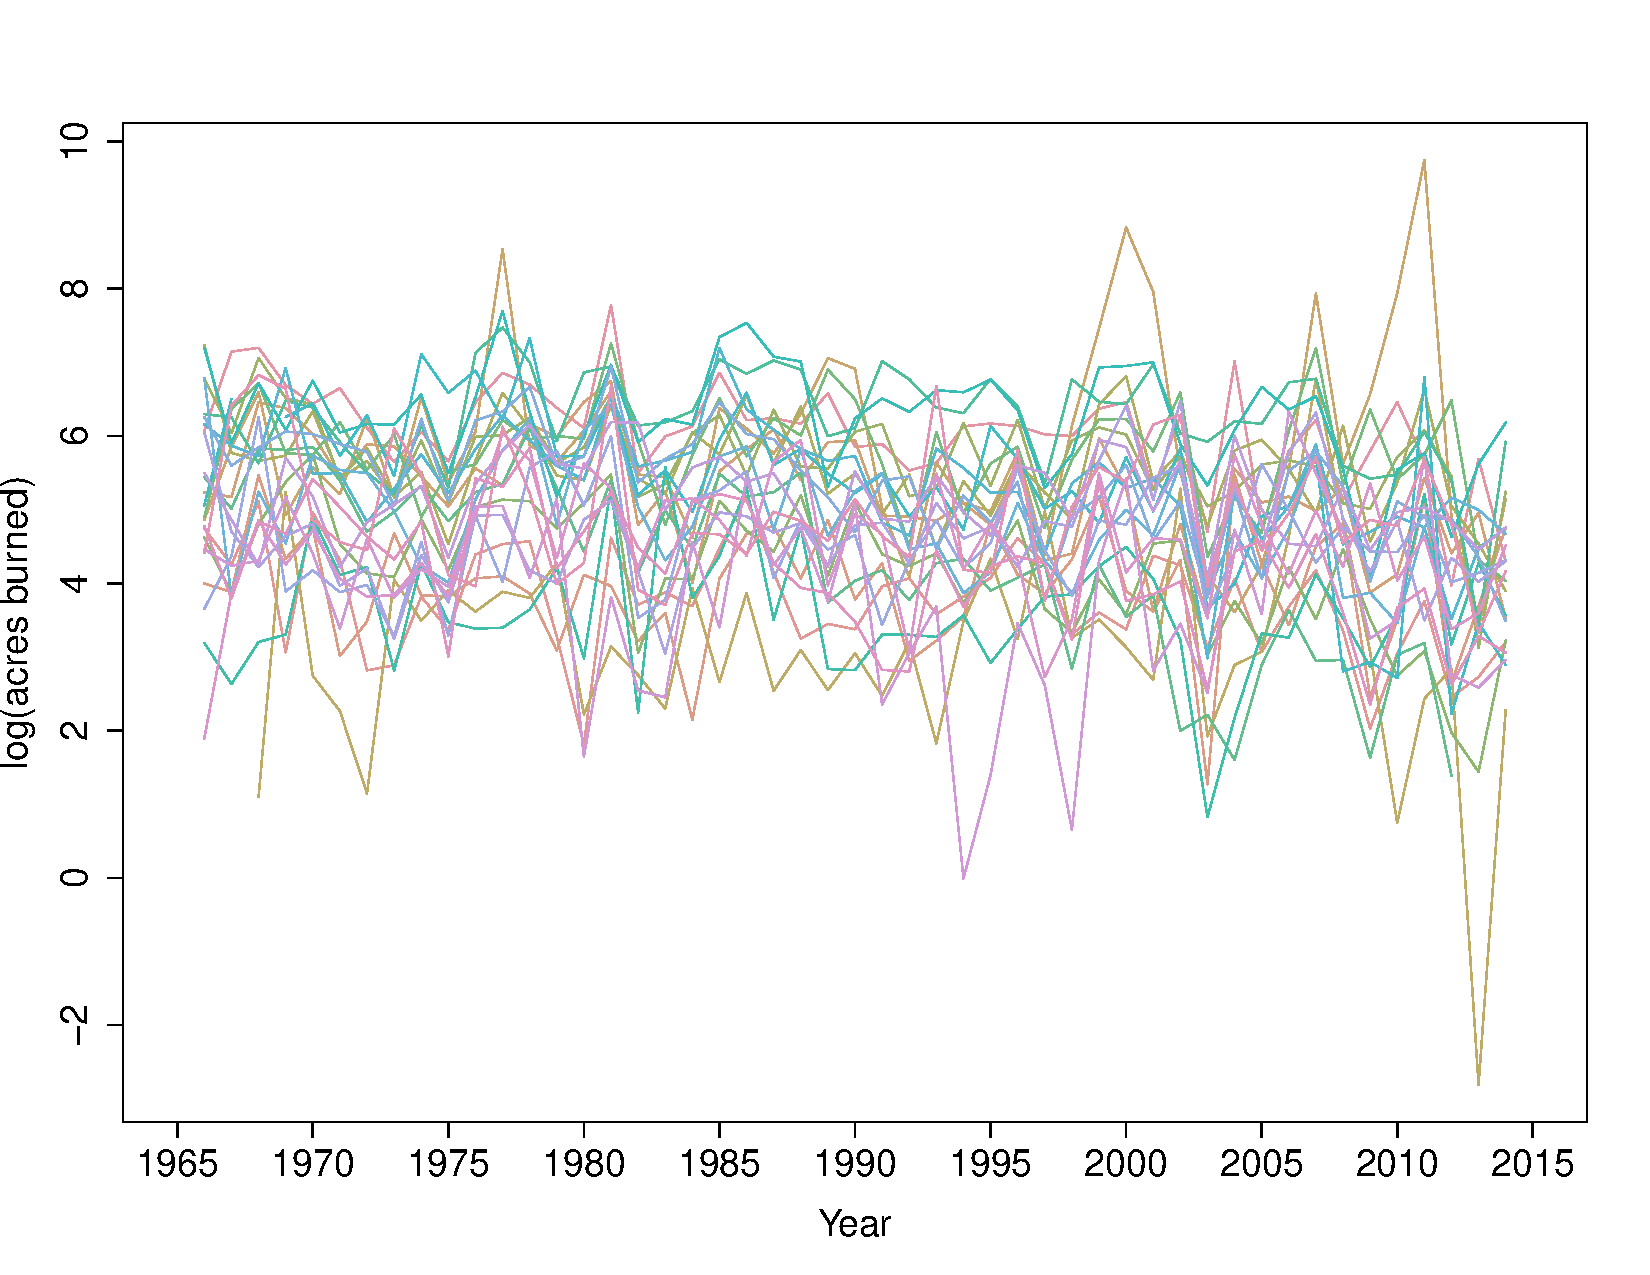
\includegraphics[width=0.80\linewidth]{plots/spag-rand-25}
  \caption{Time series of $\log$(acres burned) for 25 randomly selected counties.}
  \label{fig:firets25}
\end{figure}

We estimate the extremal coefficient function $\hat{\theta}_{ij}$ by setting $q_1 = 0.90$ and using $n_q = 100$.
With more data, it would possible to increase $q_1$, but we set $q_1 = 0.90$ to increase the stability when estimating $\hat{\vartheta}_{ij}$.

Because these data are not max-stable, we select a site-specific threshold $T_i$ to use in the analysis with the following algorithm.
Without some adjustment to the data, it is challenging to borrow information across sites to inform the threshold selection.
We first compute
\begin{align}
  \tilde{\bY}_i = \frac{\bY_i - \text{med}(\bY_i)}{\text{IQR}(\bY_i)}
\end{align}
where med$(\cdot)$ is the median, and IQR$(\cdot)$ is the inter-quartile range.
Then we combine all sites together and plot a mean residual plot for $\tilde{\bY_i}, i = 1, \ldots, n_s$.
The mean residual plot is given in Figure \ref{fig:mrlthresh}, with a vertical line indicating the quantile we use for the county-specific values $\bT$.
Based upon the mean residual plot, we select $q(0.95)$ for the spatially smoothed threshold.
To calculate $T_i$ for each county, we find $\hat{q}(0.95)$ by taking the 95$th$ quantile for county $i$ and the five closest counties.

\begin{figure}[htbp]
  \centering
  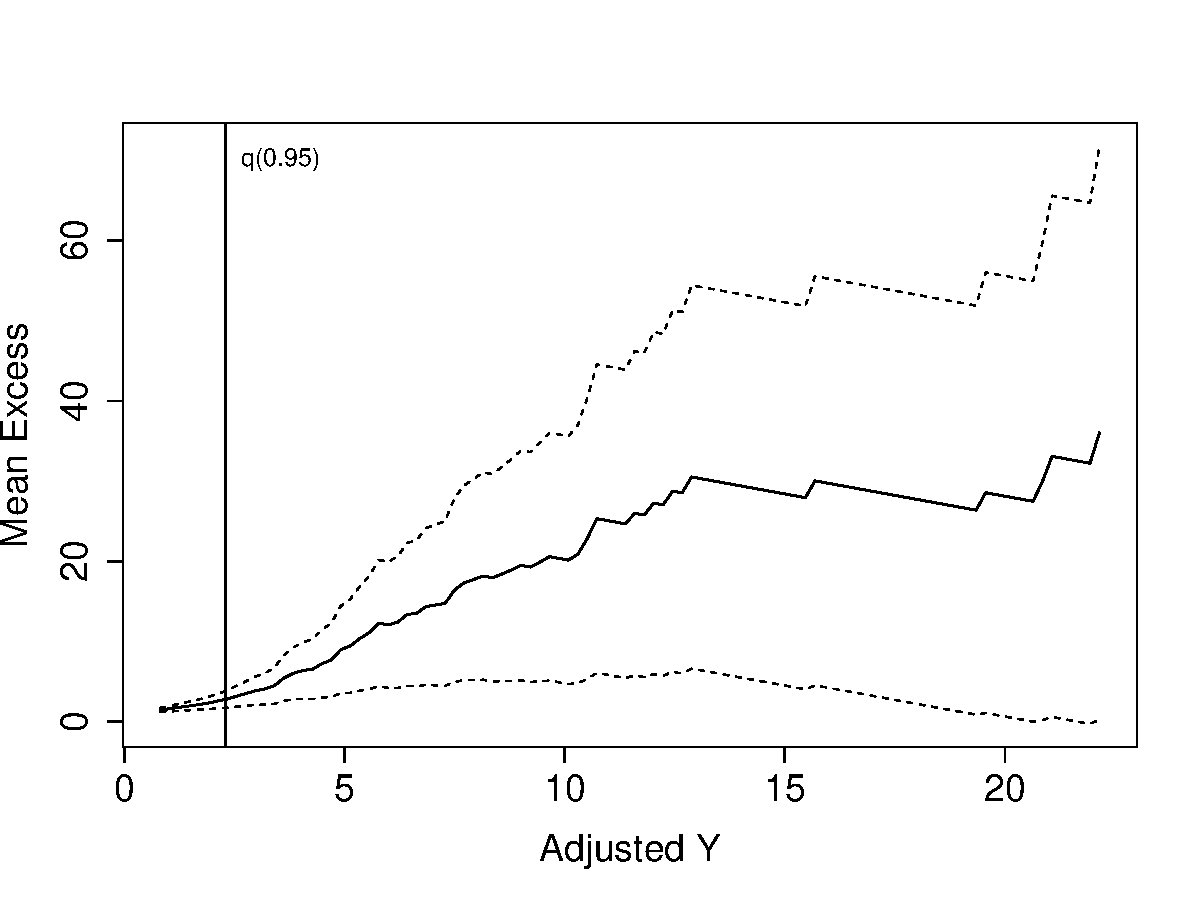
\includegraphics[width = 0.6\linewidth]{plots/mrl-zoom.pdf}  % markdown/eda/eda-plotting.R
  \caption{Mean residual plot with line indicating the $T = q(0.95)$ for the analysis.}
  \label{fig:mrlthresh}
\end{figure}

\begin{figure}[htbp]
  \centering
  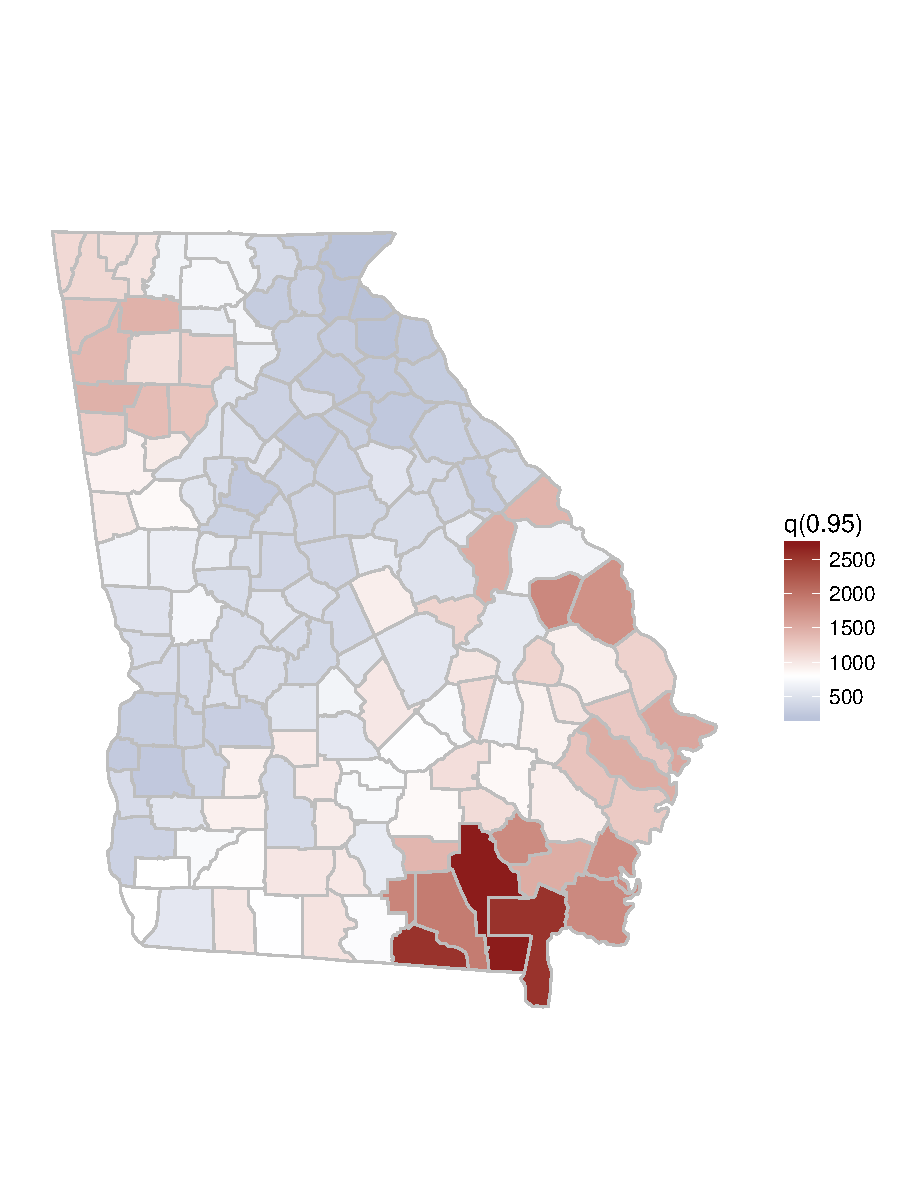
\includegraphics[width = 0.47\linewidth, trim = 0 10em 0 10em]{plots/spatial-q95.pdf}
  \caption{Spatially smoothed threshold values for each county.}
  \label{fig:mrlthresh}
\end{figure}

\subsection{Results}\label{s:results}
We use 5-fold cross-validation to assess the predictive performance of a model.
For each method, we randomly select 80\% of the observations across counties and years to be used as a training set to fit the model.
The remaining 20\% of sites and years are withheld for testing model predictions.
To assess the predictions for the test set, we use quantile scores and Brier scores \hl{citation}.
The quantile score is given by \hl{give formula}.
The Brier score is given by \hl{give formula}.
For both of these methods, we use a negative orientation, so a lower score indicates a better fit.

\begin{table}[htbp]
\caption{Average quantile scores for selected quantiles and Brier scores ($\times 1000$) for selected thresholds}
\centering
\small
	\begin{tabular}{l|rr|rr|rr|rr|rr}
	 \multicolumn{1}{c}{} & \multicolumn{2}{c}{L = 2} & \multicolumn{2}{c}{L = 5} & \multicolumn{2}{c}{L = 10} & \multicolumn{2}{c}{L = 15} & \multicolumn{2}{c}{L = 20} \\
	 \cline{2-11}
	 & Basis & Kernel & Basis & Kernel & Basis & Kernel & Basis & Kernel & Basis & Kernel \\
	 \hline
	 QS(0.95) & 157.23 & 146.18 & 156.96 & 145.07 & 151.15 & 139.47 & 147.76 & 138.49 & 147.19 & 138.35 \\
	 QS(0.99) &  93.47 &  86.27 &  90.23 &  83.43 &  88.56 &  81.29 &  85.84 &  80.14 &  86.93 &  80.57 \\
	 \hline
	 BS(0.95) &  91.61 &  84.21 &  91.45 &  84.04 &  88.43 &  82.29 &  87.57 &  81.83 &  87.17 &  81.70 \\
	 BS(0.99) &  44.63 &  41.53 &  44.55 &  41.70 &  43.18 &  40.72 &  42.81 &  40.71 &  42.43 &  40.64 \\
	 \hline
	\end{tabular}
\end{table}


\begin{figure}  % markdown/fire-analysis/combine-tables.R
	\centering
	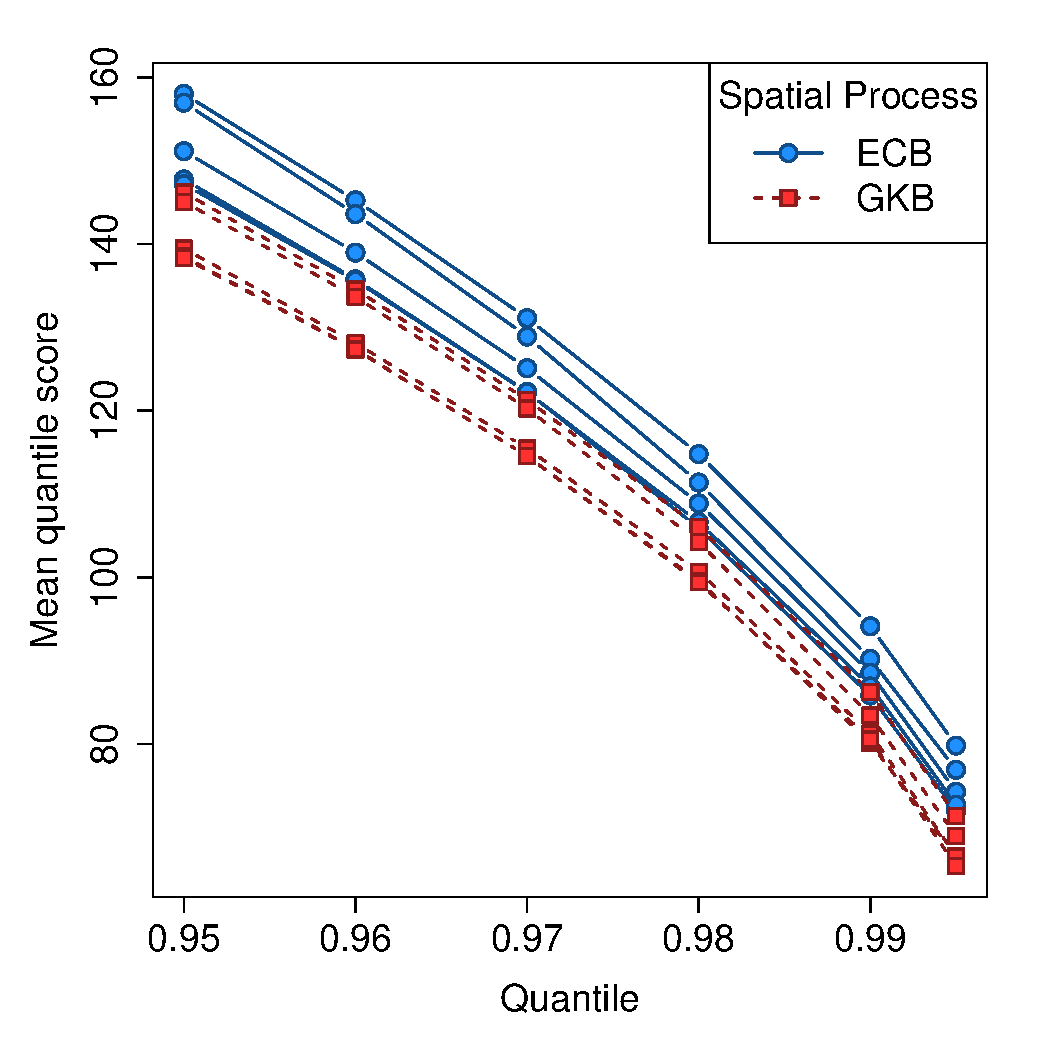
\includegraphics[width=0.47\linewidth]{plots/qs-mean}
	\caption{Average quantile score for selected quantiles}
  \label{fig:avgqscore}
\end{figure}

\begin{figure}  % markdown/fire-analysis/combine-tables.R
	\centering
	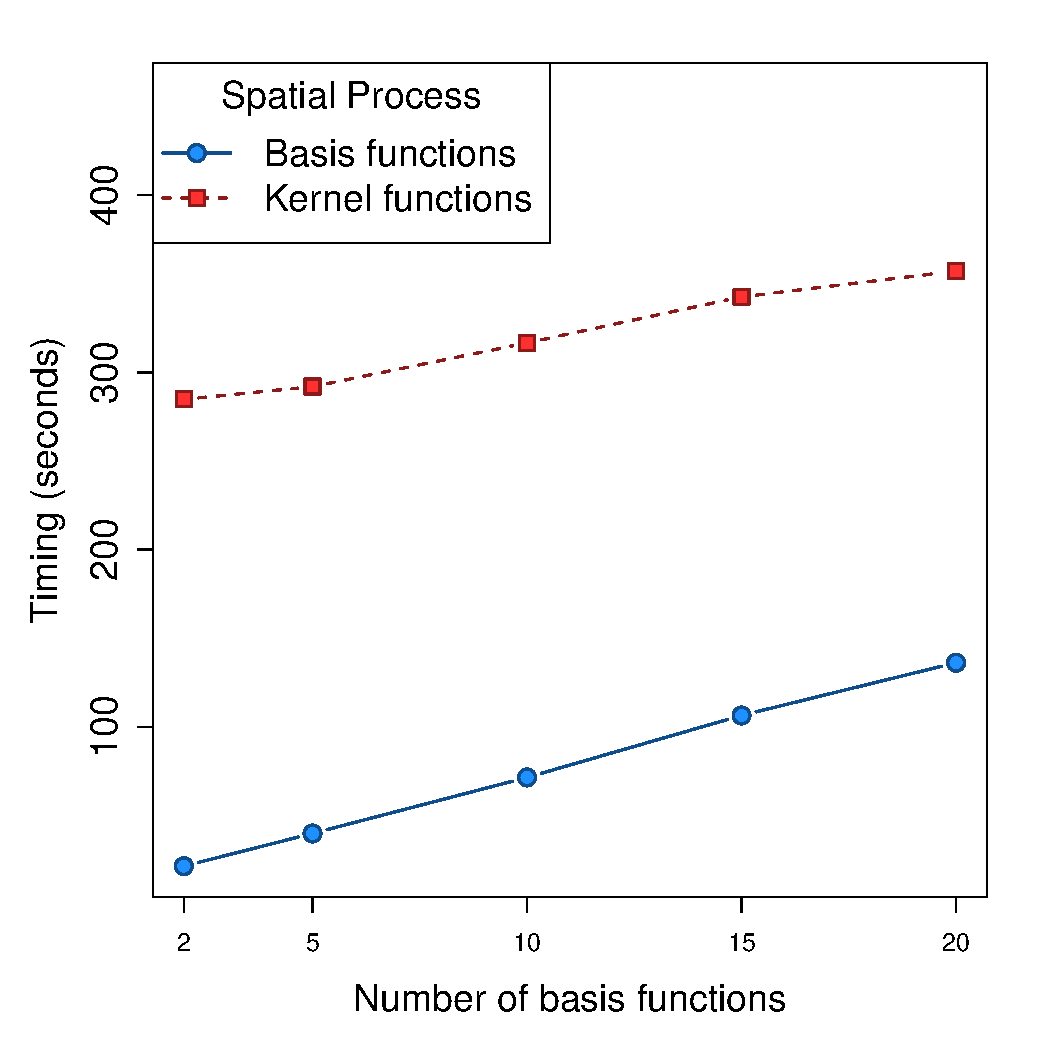
\includegraphics[width=0.47\linewidth]{plots/timing}
	\caption{Timing comparison of basis functions to kernel functions for the spatial process (100 iterations)}
  \label{fig:timingcompare}
\end{figure}

Based upon the cross-validation results, we reran the full data analysis using $L = 15$ basis functions.



\subsection{Model checking and sensitivity analysis}


\section{Conclusions}\label{s:con}

\section*{Acknowledgements}


\begin{singlespace}
\bibliographystyle{rss}
\bibliography{PCAX}
\end{singlespace}

\end{document}




